% Options for packages loaded elsewhere
\PassOptionsToPackage{unicode}{hyperref}
\PassOptionsToPackage{hyphens}{url}
\PassOptionsToPackage{dvipsnames,svgnames,x11names}{xcolor}
%
\documentclass[
  12pt,
]{article}
\usepackage{amsmath,amssymb}
\usepackage{iftex}
\ifPDFTeX
  \usepackage[T1]{fontenc}
  \usepackage[utf8]{inputenc}
  \usepackage{textcomp} % provide euro and other symbols
\else % if luatex or xetex
  \usepackage{unicode-math} % this also loads fontspec
  \defaultfontfeatures{Scale=MatchLowercase}
  \defaultfontfeatures[\rmfamily]{Ligatures=TeX,Scale=1}
\fi
\usepackage{lmodern}
\ifPDFTeX\else
  % xetex/luatex font selection
\fi
% Use upquote if available, for straight quotes in verbatim environments
\IfFileExists{upquote.sty}{\usepackage{upquote}}{}
\IfFileExists{microtype.sty}{% use microtype if available
  \usepackage[]{microtype}
  \UseMicrotypeSet[protrusion]{basicmath} % disable protrusion for tt fonts
}{}
\makeatletter
\@ifundefined{KOMAClassName}{% if non-KOMA class
  \IfFileExists{parskip.sty}{%
    \usepackage{parskip}
  }{% else
    \setlength{\parindent}{0pt}
    \setlength{\parskip}{6pt plus 2pt minus 1pt}}
}{% if KOMA class
  \KOMAoptions{parskip=half}}
\makeatother
\usepackage{xcolor}
\usepackage[margin=1in]{geometry}
\usepackage{graphicx}
\makeatletter
\newsavebox\pandoc@box
\newcommand*\pandocbounded[1]{% scales image to fit in text height/width
  \sbox\pandoc@box{#1}%
  \Gscale@div\@tempa{\textheight}{\dimexpr\ht\pandoc@box+\dp\pandoc@box\relax}%
  \Gscale@div\@tempb{\linewidth}{\wd\pandoc@box}%
  \ifdim\@tempb\p@<\@tempa\p@\let\@tempa\@tempb\fi% select the smaller of both
  \ifdim\@tempa\p@<\p@\scalebox{\@tempa}{\usebox\pandoc@box}%
  \else\usebox{\pandoc@box}%
  \fi%
}
% Set default figure placement to htbp
\def\fps@figure{htbp}
\makeatother
\setlength{\emergencystretch}{3em} % prevent overfull lines
\providecommand{\tightlist}{%
  \setlength{\itemsep}{0pt}\setlength{\parskip}{0pt}}
\setcounter{secnumdepth}{5}
\usepackage{setspace} \setstretch{1.15} \usepackage{float} \floatplacement{figure}{t}
\usepackage{bookmark}
\IfFileExists{xurl.sty}{\usepackage{xurl}}{} % add URL line breaks if available
\urlstyle{same}
\hypersetup{
  colorlinks=true,
  linkcolor={cyan},
  filecolor={Maroon},
  citecolor={Blue},
  urlcolor={cyan},
  pdfcreator={LaTeX via pandoc}}

\title{~\large Tournaments}
\author{\large Zach Culp \vspace{-1.1mm}\\
\normalsize  \vspace{-1mm}\\
\normalsize Loyola University Chicago \vspace{-1mm}\\
\normalsize Chicago, IL 60660 \vspace{-1mm}\\
\strut \\
\large Josie Peterburs \vspace{-1.1mm}\\
\normalsize \vspace{-1mm}\\
\normalsize Loyola University Chicago \vspace{-1mm}\\
\normalsize Chicago, IL 60660 \vspace{-1mm}\\
\strut \\
\large Ryan McShane \vspace{-1.1mm}\\
\normalsize Department of Mathematics and Statistics \vspace{-1mm}\\
\normalsize Loyola University Chicago \vspace{-1mm}\\
\normalsize Chicago, IL 60660 \vspace{-1mm}\\
\strut \\
\large Gregory J. Matthews \vspace{-1.1mm}\\
\normalsize Department of Mathematics and Statistics \vspace{-1mm}\\
\normalsize Center for Data Science and Consulting \vspace{-1mm}\\
\normalsize Loyola University Chicago \vspace{-1mm}\\
\normalsize Chicago, IL 60660 \vspace{-1mm}\\
\normalsize \href{mailto:ypu@something.edu}{\texttt{email}}
\vspace{-1mm}\\
\normalsize \href{mailto:zculp@luc.edu}{\texttt{zculp@luc.edu}}
\vspace{-1mm}\\
\normalsize \href{mailto:jpeterburs@luc.edu}{\texttt{jpeterburs@luc.edu}}
\vspace{-1mm}\\
\normalsize \href{mailto:rmcshane@uchicago.edu}{\texttt{rmcshane@uchicago.edu}}
\vspace{-1mm}\\
\normalsize \href{mailto:gmatthews1@luc.edu}{\texttt{gmatthews1@luc.edu}}
\vspace{-1mm}}
\date{}

\begin{document}
\maketitle
\begin{abstract}
We evaluate multiple tournament formats to assess their effectiveness in
accurately reproducing the true underlying ranking of participating
teams. Using repeated simulations for each structure, we compare teams'
true performance ranks to their simulated outcomes. To quantify the
accuracy of each format, we calculate weighted mutual information
between true and simulated rankings across a large number of replicates.
``Remarkable'' weights are applied to look at only the top n
teams/competitors in a tournament. This information-theoretic approach
allows us to objectively compare formats and identify which structures
most effectively preserve rank order. Results are visualized through
comparative plots, providing clear insights into the trade-offs and
strengths of each tournament design.\\

\vspace{2mm} \textbar{} Keywords: tournament structures, mutual
information
\end{abstract}

\section{Introduction}\label{introduction}

There are hundreds of different tournament structures that dictate how a
set of teams compete against each other to determine an overall ranking.
Different tournament structures have unique strengths and weaknesses,
affecting how well they reflect the true rankings of the teams. The goal
of a tournament is to find the best teams, but how can we quantify how
well a tournament performs? In some instances, the tournament organizers
only award the overall winner, but other times, the top three or ten
teams are awarded. Because of this, organizers may prefer one structure
over another based on their needs. Tournament organizers must also take
into account factors like cost, timeliness, entertainment value, and
fairness when choosing a tournament structure.

To evaluate a tournament's effectiveness, we propose a numerical metric
that quantifies how accurately it orders teams based on their true
rankings. Tournament results can be viewed as a ``message'' attempting
to convey the true team rankings. However, various factors introduce
noise, leading to information loss. We use principles from information
theory to measure this information loss across multiple tournament
simulations to assess the reliability of different formats.

\section{Methods}\label{methods}

Consider a set of \(n\) teams indexed from \(i = 1, 2, \cdots, n\) each
with an associated true strength parameter
\(\boldsymbol{\theta} = (\theta_1, \theta_2, \ldots, \theta_n)\) such
that \((\theta_1 > \theta_2 > \ldots > \theta_n)\). Next, let
\(r(\boldsymbol{\theta})\) be the indexes of \(\boldsymbol{\theta}\)
when theta is sorted from largest to smallest so that
\(r(\boldsymbol{\theta}) = \{1, 2, \ldots, n-1, n\}\). Next define
\(T(\phi, s)\) as a tournament with schedule \(\phi\) and seeding
structure \(s\). \(\phi\) contains all the information about the
scheduling of teams, which could be fully known prior to the tournament
(i.e.~round robin) or determined as the tournament progresses
(i.e.~single elimination tournament). We then let
\(\hat{r}(T(\phi, s),\boldsymbol{\theta})\) be an \(n\)- dimensional
vector valued random variable that gives the results of a tournament as
a vector of the indexes of the vector \(\boldsymbol{\theta}\). The index
in the first position of the vector
\(\hat{r}(T(\phi, s),\boldsymbol{\theta})\) indicates the index of the
team that finished first, the index in the second position of the vector
\(\hat{r}(T(\phi, s),\boldsymbol{\theta})\) indicates the index of the
team that finished second, and so on.

For example, in a 4 team tournament,
\(\hat{r}(T(\phi, s),\boldsymbol{\theta})\) = (3, 2, 1, 4) indicates
that the team with index 3 (i.e.~the true third best team) won the
tournament, the true second best team finished second, the true best
team finished third and the true 4th team finished 4th in that
particular tournament. If \(\hat{r}(T(\phi, s),\boldsymbol{\theta})\) =
(1, 2, 3, 4), this means that the random outcome of the tournament was
the same as the true ordering of the teams.

If one views the true ranking of the teams in a tournament as a message
to be sent to a receiver and the outcome of the tournament as a message
that is received, we can measure the ``goodness'' of a tournament in
terms of its ability to accurately transmit the true ranking. We can
then use concepts from information theory to assess the ability of a
tournament to correctly rank teams. Specifically, we start with the
concept of mutual information (CITE). For two random variables \(X\) and
\(Y\) mutual information is defined as:

\[
I(X;Y)=\sum_{y\in Y}\sum_{x\in X}p(x,y)\log \frac {p(x,y)}{p(x)\,p(y)}
\]

In our setting, we replace \(X\) and \(Y\) with
\(r(\boldsymbol{\theta})\) and
\(\hat{r}(T(\phi, s),\boldsymbol{\theta})\), and we could seek to
estimate
\(I(r(\boldsymbol{\theta}),\hat{r}(T(\phi, s),\boldsymbol{\theta}))\).
For simplicity, we drop the arguments from the functions \(r\) and
\(\hat{r}\) for ease of exposition.

We note here that \(r\) is not a random variable, however, since the
indexing of the teams in the vector \(\boldsymbol{\theta}\) is arbitrary
(we use 1, 2, 3, etc. for convenience, but any indexing is valid), we
can view this a random variable where all permutation so of the \(n\)
teams are equally likely. Therefore when calculating the mutual
information in this setting, we set \(p(r) = \frac{1}{n!}\). By a
similar argument we set \(p(\hat{r}) = \frac{1}{n!}\).

We define the mutual information of \(r\) and \(\hat{r}\) to be:

\[
I(r,\hat{r})=\sum_{r}\sum_{\hat{r}}p(r,\hat{r})\log \frac {p(r,\hat{r})}{p(r)p(\hat{r})} = n!\sum_{\hat{r}}p(r,\hat{r})\log \frac {p(r,\hat{r})}{(\frac{1}{n!})^2}
\]

While there are \(n!\) different permutations for the result of \(r\),
we don't need to sum across these as any specific choice of \(r\) is
just an arbitrary labeling of the true strength parameters vector
\(\boldsymbol{\theta}\). So given \(r\), the distribution of \(\hat{r}\)
is the same up to the labeling. Therefore, we only need to consider a
single permutation of \(r\), we compute the the quantity inside the
summation, and then multiple by \(n!\) (effectively summing across
\(r\)).

In order to compute this quantity, we need to compute \(p(r,\hat{r})\).
This probability is found by calculating the probability of a given
permutation of \(\hat{r}\) and \(r\) is assumed to be the permutation
from \(\{1, 2, \ldots, n\}\). We estimate \(p(r,\hat{r})\) empirically
through simulation.

However, using mutual information in this form does not suit our needs
in this setting. The problem is that mutual information in this form
will yield high values of mutual information when the output from the
tournament \(\hat{r}\) is highly consistent \emph{even if the ranking
from the tournament is incorrect}. As an example, if \(n=4\) and the
true order of \(\boldsymbol{\theta}\) is \(r = \{1, 2, 3, 4\}\) and
\(p(\hat{r} = \{4, 3, 2, 1\}) = 1\) will be the same mutual information
as when \(r = \{1, 2, 3, 4\}\) and \(p(\hat{r} = \{1, 2, 3, 4\}) = 1\)
and in both of these cases the mutual information will be maximized at:

\[
I(r,\hat{r})= n!\sum_{\hat{r}}p(r,\hat{r})\log \frac {p(r,\hat{r})}{\left(\frac{1}{n!}\right)^2} = n! log((n!)^2)
\] and for the specific case when \(n=4\) would be: \[
4! log_2(4!^2) = 24*log_2(24^2) = 220.0782
\]

In order to alleviate this problem, we instead consider \emph{weighted}
mutual information. We want to give more weight to permutations from
\(\hat{r}\) that are ``closer'' to \(r\). There are any number of
reasonable choices for this weighting function, and we choose to use
squared error. Specifically,

\[
w(r, \hat{r}) =
\begin{cases}
\frac{1}{\hat{r}'r}, & r \ne \hat{r} \\
1, & r = \hat{r}
\end{cases}
\]

In general, though any loss function \(l(r, \hat{r})\) can be used:

\[
w(r, \hat{r}) =
\begin{cases}
\frac{1}{l(r, \hat{r})}, & r \ne \hat{r} \\
1, & r = \hat{r}
\end{cases}
\]

Note that one is 1/N!

And this does work because consistently getting the order incorrect is
perfect information.

However, because the number of teams that need to be accurately ordered
differs based on the tournament organizers, a second weighting function
was found to portray the importance, or remarkability, of each value in
\(\hat{r}\). We call these ``remarkable weights'' (\(m(r)\)) to
differentiate from the other weighting function. ``Remarkable weights''
are set to allow for a subjective belief of what determines a good
tournament. For a four-team tournament, if the user decides that only
the winner is important, then \(m(r) = \{1,0,0,0\}\). However, if the
organizers want an accurate leaderboard with the winner as the most
important, then a potential \(m(r)\) could be \(\{3,1,1,0\}\). With the
addition of the weighting functions, the formula for mutual information
is updated:

\[
I(X;Y)=\sum_{r}\sum_{\hat{r}} w(r,\hat{r}) * m(r) * p(r,\hat{r})\log \frac {p(r,\hat{r})}{p(r)p(\hat{r})}
\]

Because this mutual information is unitless, the formula can be
standardized to be between 0 and 1 using the complement of Rajski's
distance: \[
1 - (1 - \frac{I(X,Y)}{\text{max\{}H(X), H(Y)\}})
\]

where \(H(X,Y)\) is entropy given by:

\[
max\{H(X), H(Y)\} = \sum_{r}  p(r) \log p(r) = n! \log n!
\]

The complement is taken so that the more accurate tournaments are closer
to 1 and the less accurate are closer to 0.

\section{Results}\label{results}

In order to fairly compare tournament structures, we assume the true
strengths of the teams follow a normal distribution, where each team is
assigned an equally spaced quantile and each team's strength is the
z-score of its respective quantile. Using this assumption, 10,000
simulations, all with 8 total teams, were ran for a single game round
robin (each team plays each other once), a single elimination structure
with the usual seeding structure (1 vs 8, 4 vs 5, 3 vs 6, 2 vs 7), a
single elimination structure with a poor seeding structure (1 vs 2, 3 vs
4, 5 vs 6, 7 vs 8). For a better understanding of the results, the best
possible results (every structure has the best in rank 1, the 2nd best
in rank 2, etc), the worst possible results (every structure has the
worst in rank 1, the 2nd worst in rank 2, etc), every possible
permutation of the ranks once, and a single elimination tournament with
the usual seeding structure where every team is of equal strengths.
Because the metric found is unitless, we were able to normalize the
values using the best and worst results to make the range from 0 to 1,
with 0 as the worst and 1 as the best. After normalizing, we get the
following graph (note the y-axis is on a log10 scale):

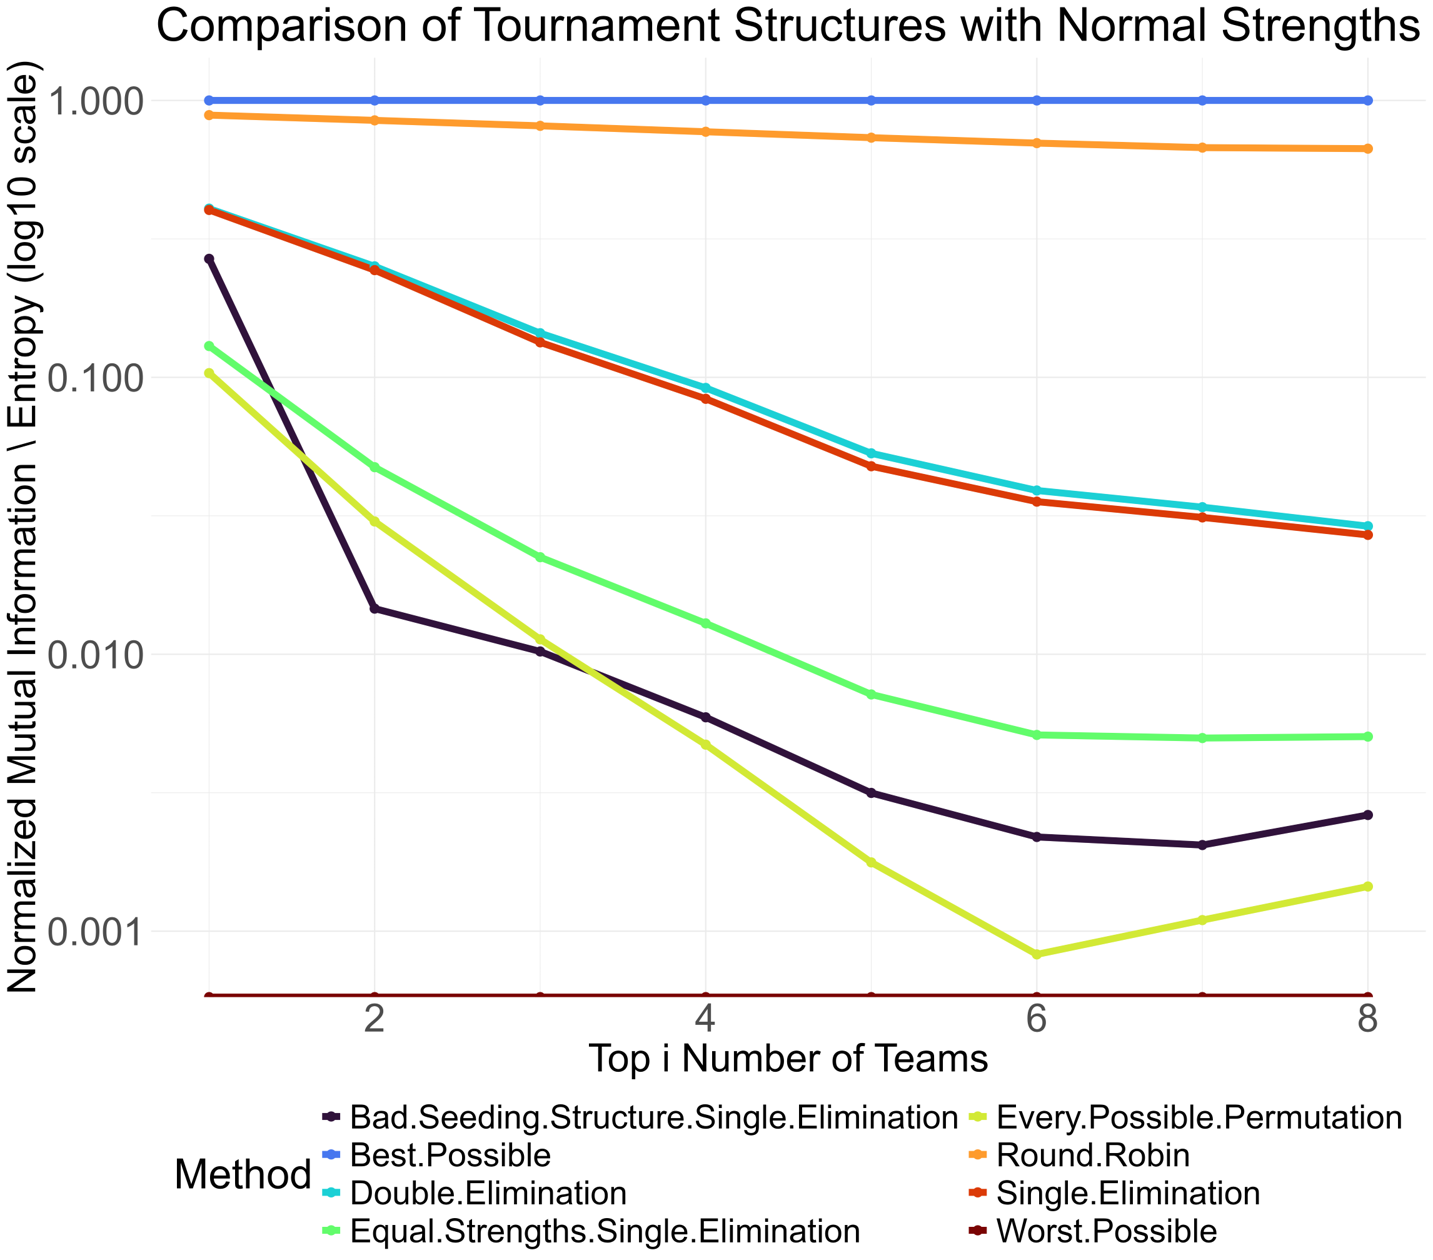
\includegraphics[width=4.25in,height=\textheight,keepaspectratio]{images/Normal_Information_Curve_Graph.png}

Based on the graph, the intuitive best tournament, round robin, does
show to be the best. Double elimination is slightly better than single
elimination, with the gap growing wider as the top number of teams
looked at increases. However, those are under the assumption that the
true strengths were ordered correctly in the seeding. If there is a poor
seeding structure, as seen in the graph, it can drastically impact the
effectiveness of the tournament. In the extreme case seen, the
tournament can actually become worse than deciding games by random
chance (like flipping a coin). Another important discovery is that the
single elimination structure with equal strengths is better than every
possible permutation. The line for every possible permutation would
likely be similar to a round robin structure with all equal strengths,
so perhaps the closer the teams are in true strength, the closer round
robin and single elimination become.

\section{Conclusion}\label{sec:conclusion}

This study introduced a weighted mutual information framework to
evaluate the effectiveness of different tournament formats in preserving
the true underlying rankings of teams. By simulating tournaments with
varying seeding structures and applying an information-theoretic
approach, we quantified how accurately each format conveys ranking
information. Our findings confirm the intuitive advantage of round robin
tournaments, which consistently outperformed single and double
elimination formats in ranking accuracy. Additionally, we observed that
seeding plays a critical role: poor seeding structures can significantly
degrade performance, in some cases making outcomes less informative than
random chance.

These results underscore the trade-off between tournament accuracy and
practical constraints such as time, cost, and entertainment value. While
round robin offers the highest fidelity to true rankings, it is often
impractical for large tournaments, highlighting the need for hybrid or
adaptive structures that balance accuracy with logistical feasibility.

Future work should extend this analysis to scenarios with more
tournament structures, more teams, incorporate probabilistic strength
models reflecting real-world uncertainty, and explore alternative
weighting schemes for different competitive priorities (e.g., top-4
accuracy versus full ranking). Applying these methods to actual
tournament data could further validate their usefulness for organizers
aiming to design fair and informative competitions.

\section*{Acknowledgements}\label{acknowledgements}
\addcontentsline{toc}{section}{Acknowledgements}

We thank the Department of Mathematics and Statistics at Loyola
University Chicago for their support and resources in conducting this
study. No external funding was received for this research.

\section*{Supplementary Material}\label{supplementary-material}
\addcontentsline{toc}{section}{Supplementary Material}

All supplementary material available at
\url{https://github.com/gjm112/tournaments}.

\section{References}\label{references}

Rajski, C. (1961). ``A metric space of discrete probability
distributions''. Information and Control. 4~(4):~371--377.
\url{doi:10.1016/S0019-9958(61)80055-7}.

McShane, R. (2019). \emph{Modeling Stochastically Intransitive
Relationships in Paired Comparison Data.} (Doctoral dissertation).
Southern Methodist University. Retried from
\url{https://scholar.smu.edu/hum_sci_statisticalscience_etds/13/}

Karel Devriesere, László Csató, Dries Goossens (2024). ``Tournament
design: A review from an operational research perspective''. European
Journal of Operational Research.
\url{https://doi.org/10.1016/j.ejor.2024.10.044}.

\end{document}
